\section{Background}
\label{src:bground}

In this section, we provide a brief introduction to Cray SHMEM and an
overview to the existing memory model in the OpenSHMEM standard
specification.

\subsection{OpenSHMEM}
\label{src:bg/osm}
OpenSHMEM is a Partitioned Global Address Space~\cite{pgas} (PGAS) library
interface specification which is a culmination of a unification effort
among various vendors and users in the SHMEM programming community. It
provides an Application Programming Interface (API) for the SHMEM libraries
to support one-sided point-to-point data communication with a chief aim of
performance and portability. It follows an SPMD-like execution model, where
all the processes or Processing Elements(PEs) are launched at the begining
of the prohram; each PE executes the same code and the number of PEs remains
unchanged during the execution of the program. The main features of OpenSHMEM
API includes the support for:
\begin{itemize}
    \item remote memory access through one-sided point-to-point blocking and
    non-blocking communication for both continguous and strided data transfers;
    \item atomic memory operations;
    \item collective communication;
    \item synchronization and memory ordering; and
    \item mutual exclusion through distributed locking
\end{itemize}

\subsection{Cray SHMEM}
\label{src:bg/crayshmem}
There are various production-grade, closed source OpenSHMEM implementation as well
as open source implementations available. Cray SHMEM~\cite{csma} is a vendor-based
closed source OpenSHMEM implementation from Cray Inc., available as part of the Cray
Message Passing Toolkit~\cite{mpt} (MPT). It is implemented over DMAPP~\cite{dmapp},
an optimized communication layer for Cray architectures. Cray SHMEM is OpenSHMEM
specification version-1.3~\cite{osm13} compliant. Apart from the OpenSHMEM standard
specific features, it provides support for the following features as \texttt{SHMEMX}
prefixed extensions:
\begin{itemize}
    \item thread-safety in OpenSHMEM extensions;
    \item put with signal communication;
    \item OpenSHMEM PE subsets called as Teams; and
    \item Team-based collective communication extensions;
\end{itemize}

\subsection{OpenSHMEM Memory Model}
\label{src:bg/mmodel}
Based on accessibility, any OpenSHMEM program consists of two types of data
objects; remotely accessible and private data objects. The private data objects
are local to a particular PE and are accessible by only that particular PE.
These local data objects follow the same memory model of the base programming
language (C or Fortran). The remotely accessible data objects are accessible
by any PE using the OpenSHMEM extensions and they are called as \emph{Symmetric
Data Objects}. Each symmetric data objects has a corresponding object with same
name, size and data type on all PEs. A data object is considered a symmetric
data object if it is a:
\begin{itemize}
    \item global or static variable on C/C++ and not defined in DSO; and
    \item data allocated by \texttt{shmem\_malloc} or \texttt{shpalloc}
    OpenSHMEM extensions on C/C++ and Fortran language respectively
\end{itemize}

The data allocated by \texttt{shmem\_malloc} and \texttt{shpalloc} collective
OpenSHMEM extensions are placed on a special memory region called \emph{Symmetric
Heap}. There is one symmetric heap on every PE created during the program execution
on a memory region determined by the OpenSHMEM implmentation. It may reside on
different memory regions on different PEs. Except the size of the symmetric heap
determined by \texttt{SMA\_SYMMETRIC\_SIZE} environmental variable, users have no
other control on the symmetric heap.

\begin{figure}[!h]
    \vspace{-20pt}
    \hspace*{5mm}
    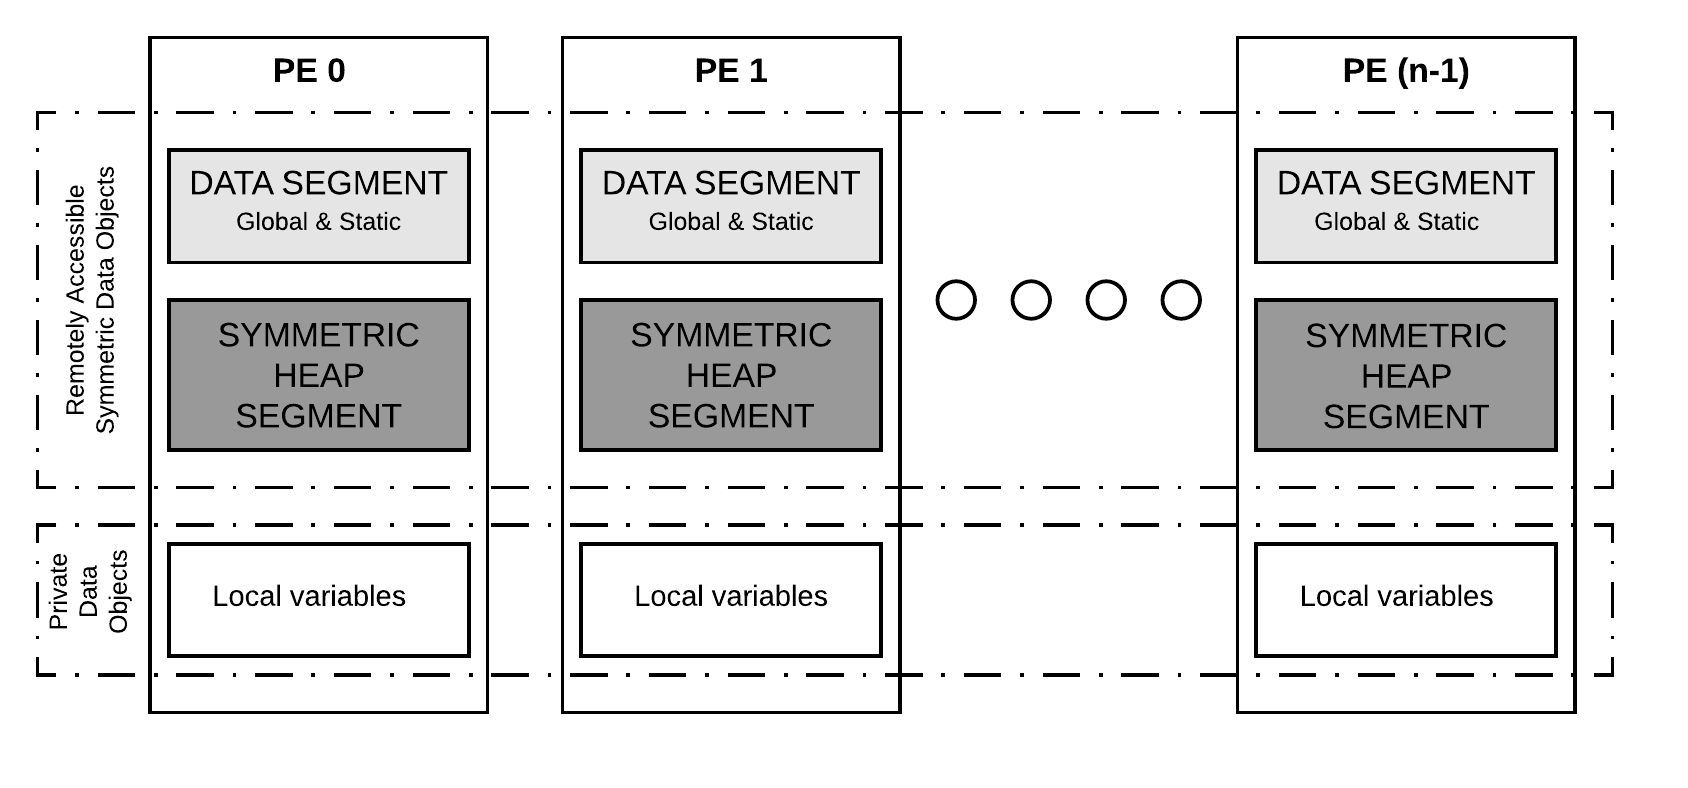
\includegraphics[scale=0.20]{image/osm-mmodel.png}
    \vspace{-25pt}
    \caption{OpenSHMEM Memory Model}
    \label{fig:mmodel}
\end{figure}

Figure~\ref{fig:mmodel}, shows the type of different data objects available in
OpenSHMEM. Global and Static variables are allocated on the \emph{data segment},
while the the variable with data allocated using \texttt{shmem\_malloc} and
\texttt{shpalloc} extensions are placed on the \emph{symmetric heap segment}.
Variables on both the data and symmetric heap segments are remotely accessible.
Figure~\ref{fig:mmodel} also shows that there is only one symmetric heap segment
per PE. Local variables are allocated on the local data objects which retains the
same memory model from the underlying base language.